\section{System Model}\label{sec_system}
Figure~\ref{fig_system} illustrates the system model in consideration which consists of AUTOSAR software applications \ttsexp{A}{a}[k] partitioned on an execution platform such as the computing units \ttsexp{N}{n}[h] and the shared network bus $B$. The applications have user-defined requirements $A\rightarrow (\mathrm{RL,EE,CL})$ respectively, reliability goals (or requirement), end-to-end timing requirements, and criticality levels. The execution platform has  provisions (or capabilities) $\{N,B\}\rightarrow (\mathrm{HZ,PW,FR})$ respectively, the processor speed of computing units, the power-consumption specification and failure rates of computing units and the network bus.
 \begin{figure}[!h]
	\centering
	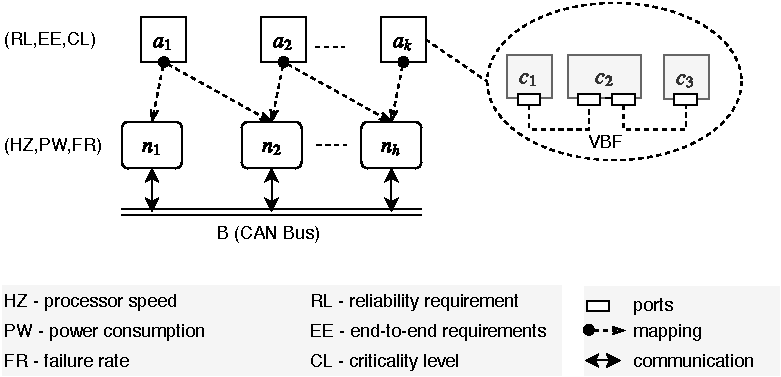
\includegraphics[scale=0.8]{system_model2}%softwareallocation
	\caption{System Model.}
	\label{fig_system}
\end{figure}
%The end-to-end timing requirements are the timing constraints over the end-to-end functional behaviors of the applications. These requirements are often specified on the \textit{cause-effect chains} consisting of software components and (potentially network messages) within the application. The reliability requirement is the expected reliability goal over a period of time $t$ in which no failure of the application experienced, and the criticality level signifies the importance of an application over other applications that have lower criticality levels, thus prioritizing the application during resource contention. The criticality levels are defined systematically, e.g., following the hazard analysis according to the ISO 26262 standard for functional safety in road vehicles~\cite{iso201126262}. 

\paragraph{Notations} For easy reading, we introduce the main notations used throught the paper as follows:

\begin{longtable}{@{}llp{0.5\textwidth}@{}}
\toprule	\small
 & Notation                        & Description                                             \\ 
\midrule
 &/* Application related */&\\
$\bullet$ & \multicolumn{2}{p{0.8\textwidth}}{\ttsexp{A}{a}   denote software applications, modeled as directed acyclic graphs of runnables, where $\mathcal{V}(a_k)$ are the nodes and $\mathcal{E}(a_k)$ the directed edges of the graph $a_k$.*}\\
$\bullet$ & \sexpsp{C}{c}     		             & software-component types used in \ttar\\
$\bullet$ & \sexpss{Q}{q}    		            & component replicas of type \ttsss{c}\\
$\bullet$ & \sexpss{R}[i]{r}[j]   	             & runnables of \ttsss{c}\\
$\bullet$ & \sexpss{T}[i]{r}[j]   	             & tasks mapped to \ttsss{c}\\

&/* Execution platform related */ &\\
$\bullet$ & \ttsexp{N}{n}         	            & computation (or computing) nodes      \\
$\bullet$ & \ttsexp{M}{m}         	           & messages on the CAN bus   \\
$\bullet$ & \multicolumn{2}{p{0.8\textwidth}}{$\tau,c,m,\gamma$ denote iterator variables,  respectively for task, component, chain and node, e.g., $\forall \tau \in  \sss{T}$ of \ttsss{c}.}\\
 &/* Mapping related */&\\

$\bullet$ & \ttsexp{\textbf{x}}{\textbf{x}}[k]         & a mapping vector from \ttssp{Q} to $M$             \\
$\bullet$ & \multicolumn{2}{p{0.8\textwidth}}{$k,i,j$ denote iterator index-variables,  respectively for the mapping vector \ttx, and rows and columns of the matrix \ttxsp{k}, e.g., \ttxkij.***}\\
$\bullet$ & \multicolumn{2}{p{0.8\textwidth}}{$\sexp{B}{b}$   directed acyclic graphs of tasks, where $b_k$ refines $a_k$ using merging rules.} \\
$\bullet$ & \sexpsp{\Gamma}{\Gamma}  & end-to-end chains             \\
$\bullet$ & \ttsss{\Gamma}$=(e_i)_{i=1}^Z$   & a chain of $e\in V(\sss{g}[k][\tau])\cup M$\\ 
&/* Functions related */ &\\

$\bullet$ & $Power(\textbf{x})$                		& total power consumption of  $A$ in \ttx    \\
$\bullet$ & $Reliability_{a}(\x)$      					& application reliability  of $a\in A$ in \ttx              \\
$\bullet$ & $ResponseTime_{\tau}(\x)$     		& response time of  $\tau \in V(\sss{g}[k][\tau])(\x)$                       \\
$\bullet$ & $Delay_\gamma(\x)$            			& age delay of $\gamma \in \ssp{\Gamma} $   in \ttx     \\
\bottomrule\\
\end{longtable}
{\footnotesize 
	*Note: the total elements in a set $S$ is denoted by \ttn{S}, e.g., \ttn{A} denotes the number of applications in the set $S$, essentially it refers to its cardinality.\\
   *** For other uses of the iterators, they are defined in the context.}

\subsection{Software Applications}
A software application represents an independent and self-contained user-defined software functionality, e.g., x-by-wire, electronic throttle control, flight control, etc. In AUTOSAR, software applications are developed using a \textit{Software Component} (SW-C), which is design-time concept that represents the lowest-level hierarchical element in software architecture of the software application, hence is atomic. Consequently, a software component is mapped to single computing unit. It is implented by the AUTOSAR runnables, which are schedulable pieces of codes (or objects), and contains specifications of timing behavior as well as resources requirements of the runnables. We formall represent an AUTOSAR software application as follows:

\begin{definition}[AUTOSAR Software Application]\footnote{ Note: only relevant concepts of the official AUTOSAR software application definition is assumed to avoid unnecessary complexity. }\label{def_application}
We represent a AUTOSAR software appplication a \textit{directed acyclic vertex-weighted} graph $\langle V, L, w, \rangle$ of periodic runnables, where $V$ denote runnable nodes, $a_{ij}\in L$ a data-dependency link from $r_i$ to $r_j$, where $i \neq j$. The assignment function $w: V\rightarrow (\mathrm{E}_i\mathrm{,D,P, N})$ sets each runnable nodes the computation cost such as worst-case execution times (WCET) $\mathrm{E=\{E}_h:h=1,...,n_N\}$, deadline D and period P, where $\mathrm{E}_h\in \mathrm{E}$ is the WCET of $r$ on the computing unit $n_h\in \mathcal{N}$.
\end{definition}
\begin{figure}
	\centering
	\begin{minipage}{.475\textwidth}
		\centering
	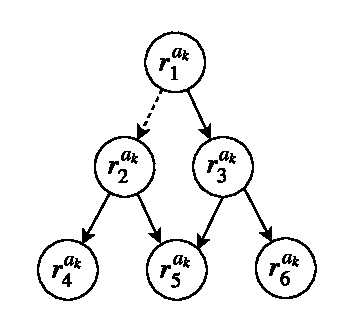
\includegraphics[width=0.7\linewidth]{img/dag_runnables}
	\caption{A Software Application Modeled as Directed Acyclic Graph.}
	\label{fig_dagcomp}
	\end{minipage}\hfill
	\begin{minipage}{0.475\textwidth}
		\centering
			\begin{tabular}{@{}llll@{}}
			\toprule
		\ttsss{c}& \ttsss{r}[k][j] &$(\mathrm{E}_h, \mathrm{P=D})$ & $\prec$ \ttsss{r} [k][i]\\ \midrule
		1&1 & $(0.1,10)$   & 2 \\ 
		2&2 & $(0.1,20)$ &  \\ 
		2&3 & $(0.1,15)$ &  \\ 
		2&4 & $(0.1,8)$   &  \\ 
		3&5 & $(0.1,12)$  &  \\ 
		3&6 & $(0.1,6)$   &  \\ 
		\bottomrule 
	\end{tabular}
		\caption{Runnables Timing Specifications.}
		\label{tbl_runnables_specs}
	\end{minipage}
\end{figure}


A path in the graph $\sss{\Gamma}=(r_i)_{i=1}^l=r_1\rightarrow,...,\rightarrow r_l$ represents a \textit{cause-effect} chain, where $r_1$ is the source of chain and $r_l$ the sink, e.g., from the appication \ttar[1]in Figure~ \ref{fig_dagcomp}, $\ssb{r}[1,1]\rightarrow \ssb{r}[2,1]\rightarrow \ssb{r}[2,3]$ is the chain, and $\ssb{r}[1,1],\ssb{r}[2,3]$, respectively are the source and the sink of the chain. A chain is a sub-functionality of the application that is triggered by a stimulus (or stimuli), e.g., pressing a brake pedal, and the corresponding response, e.g.,  vehicle braking to the desired speed level. It usually has a user-defined timing requirement, known as \textit{end-to-end} timing requirement (EE), which puts an upper-bound on the duration between the stimulus and the corresponding response of executing the chain. The set of chains in \ttar are represented as \sexpsp{\Gamma}{\Gamma}. We assume each runnable is subscribes to at least one chain.

\subsection{Scheduling Software Applications}
We assume software applications share the execution platform such as the computing units and the on-board network bus, following the mixed-criticality design~\cite{Vestal2007PreemptiveAssurance}. Thus, software applications with different software criticality should be isolated in order to prevent interference of lower-criticality applications on higher-critical applications. Assume the braking functionality of a vehicle, which is safety-criticality, is distributed over multiple computing units. Another application with infotainment functionality also shares the computing units The mixed-criticality design to this problem ensures both applications are schedulable during absence of errors, however, the braking application must also be schedulable in cases of overrun due to errors, e.g., by degrading or inhibiting the infotainment application. There are several techniques in the literature that deal with the scheduling of mixed-criticality applications on \textit{uniprocessor} systems \cite{Vestal2007PreemptiveAssurance}. In this work, we consider the \textit{partitioned criticality (PA)} (or criticality-as-priority assignment, CAPA) technique to schedule the mixed-criticality applications, which prioritizes applications based on criticality, rather than \textit{deadline} as used by the deadline monotoic assignment \cite{Baruah2011Response-timeSystems}. In contrast to other techniques, CAPA effectively counters \textit{criticality inversion}, that is unbounded blocking of higher-criticality applications by lower-criticality applications, and does not require a runtime monitoring of applications, e.g., using servers \cite{AbeniIntegratingSystems,Ashjaei2017DesigningSystems,Inam2014ThePlatforms}, albiet inefficient\footnote{Note: scheduling techniques other than the PA technique can be used with our approach to schedule the applications.}. 

The AUTOSAR software  applications are schedulable if the runnables, messages, and chains in the distributed system are schedulable, that is meet their corresponding deadlines. According to AUTOSAR~\cite{AUTOSAR2017SpecificationSoftware}, runnables are high-level schedulable objects that are mapped to tasks subsequently scheduled by AUTOSAR operating system \cite{bibid}. Thus, next, the mapping of runnables to tasks, and  schedulability of tasks and chains are explained.

\subsubsection{Runnables-to-Tasks Mapping/Transformation}\label{subsec_runnables-to-tasks}
In the mapping process, one or more runnables can be merged to optimize the runtime execution by reducing the number of schedulable tasks. Thereore, through the mappings, eventually runnable graphs are refined by task graphs as shown in Figure~{\ref{fig_appexample} (b). Moreover, the end-to-end timing analysis of chains are also defined on task chains. In this work, the following rules are applied in order to merge any runnables $a,b\in \gr{V}{\ar}$ to $v\in \gr{V}{\at}$, that is only if the following rules satisfy:
\begin{enumerate*}[label=(\roman*)]
	\item the runnables are co-hosted in the same computing unit, that is $a\mapsto n \land b\mapsto n$, where $n\in N$;
	\item activation periods of $a$ is a factor of $b$, or viceversa, and the sum of worst-case execution times of the runnables is less than the minimum of the periods.
\end{enumerate*}.
	
If the rules are satisfied, the task's timing specifications are set as follows: 
\begin{enumerate*}[label=(\roman*)]
	\item the WCET of the task is set to the sum of the WCET of the runnables, E$_h^v=$E$_h^a + $E$_h^b$, where $h:1,...,n_N$;
	\item the period and deadline of the task is set to the minimum periods of the runnables, P$_v$=D$_v=min($P$_a, $P$_b)$;
	\item otherwise, runnables are not merged, instead, each runnable that is not merged is mapped to a task while preserving the timing specifications of the runnables.
\end{enumerate*}
\begin{figure}
\vspace{0pt}\raggedbottom
	\begin{minipage}{.475\textwidth}
		\centering
		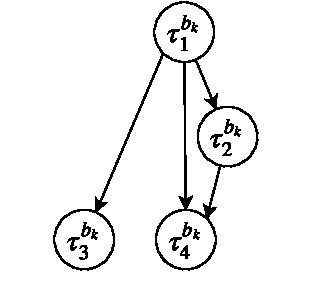
\includegraphics[width=0.6\linewidth]{img/dag_tasks}
		\caption{A Software Application Modeled as Directed Acyclic Graph.}
		\label{fig_dag_tasks}
	\end{minipage}%
\hfill
	\begin{minipage}{0.475\textwidth}
	\centering
		\begin{tabular}{@{}lll@{}}
						&&\\
			&&\\
			\toprule
			\ttsss{\tau}&$\bigcup\sss{r}[k][j]$&$(\mathrm{E}_h, \mathrm{P=D})$ \\ 
			\midrule
			1 & 1,2 &  $(0.2,10)$\\ 
			2& 3 &  $(0.1,15)$\\ 
			3& 4&  $(0.1,8)$\\ 
			4 & 5,6 &  $(0.1,6)$\\ 

			\bottomrule 
		\end{tabular}
		\caption{Tasks Timing Specifications after Merging.}
		\label{tbl_tasks_specs}
	\end{minipage}
\end{figure}

%\begin{figure}
%	\centering
%	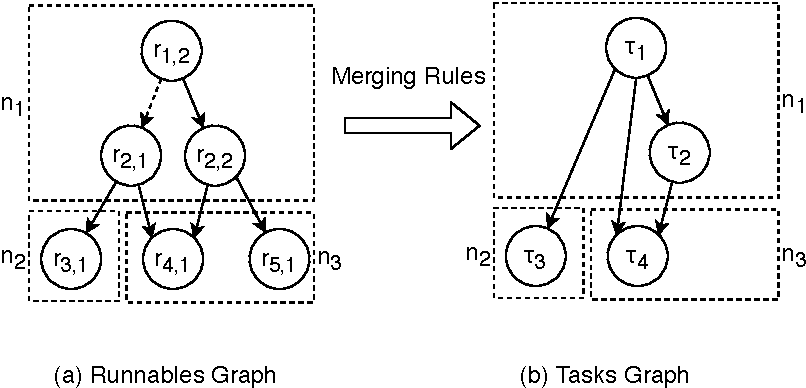
\includegraphics[width=0.7\linewidth]{img/runnable_task_dag}
%	\caption[Example of a Software Application.]{Example of a Software Application, Modeled as Directed Acyclic Graph, where $\dashrightarrow$, $\dashrightarrow$ denote triggering link, data-flow link, respectively.}
%	\label{fig_appexample}
%\end{figure}
%
%\begin{table}
%	\parbox{.45\linewidth}{
%		\centering
%		\begin{tabular}{|c|c|c|c|}
%			\hline 
%			\ttsss{r}[k][i,j] &$m_h$& $(e_h, P)$ & $\prec$ \ttsss{r} [k][i,j]\\ 
%			\hline 
%			1,1 & 1&$(1,10)$ & 2,1 \\ 
%			\hline 
%			2,1 &1& $(1,5)$ &  \\ 
%			\hline 
%			2,2 &1& $(1,15)$ &  \\ 
%			\hline 
%			3,1 & 2&$(1,20)$ &  \\ 
%			\hline 
%			4,1 & 3&$(1,10)$ &  \\ 
%			\hline 
%			5,1 & 3&$(1,20)$ &  \\ 
%			\hline 
%		\end{tabular} 
%		\caption{Runnables Timing Specifications.}
%	}
%	\hfill
%	\parbox{.45\linewidth}{
%		\centering
%		\begin{tabular}{|c|c|c|}
%			\hline 
%			\ttsss{\tau} &$\bigcup\sss{r}[k][i,j]$& $(e_h,P)$ \\ 
%			\hline 
%			1 & 1,2;2,1 &  $(2,5)$\\ 
%			\hline 
%			2& 2,2 &  $(1,15)$\\ 
%			\hline 
%			3& 3,1 &  $(1,20)$\\ 
%			\hline 
%			4 & 4,1;5,1 &  $(1,10)$\\ 
%			\hline 
%		\end{tabular} 
%		\caption{Tasks-Runnables Mappings.}
%	}
%\end{table}



\subsubsection{Scheduling Tasks and Messages}\label{subsec_response-time_analysis}
We assume tasks are scheduled using the \textit{fixed-priority preemptive scheduling polity} (FPPS)~\cite{Sha-RTS-2004}. Initally, applications are priortized based on their criticality levels followng the PA technique, and within each application the tasks are prioritized according to the \textit{deadline monotonic} (DM) priorities assignment. 
\[
cri(b_i)>cri(b_j)\implies \forall \tau_1,\in V(b_i)\forall \tau_2\in V(b_j)\ Pri(\tau_1)>Pri(\tau_2),
\]
where $\forall i,j:1,...,n_A\land i\neq j$, $cri$ and $pri$ are predicates which detemine the critiality and priority of tasks $\tau_1,\tau_2$, respectively; $V(b_i), V(b_j)$ are returns the tasks nodes, respectively for $b_i$ and $a_j$.

The schedulability of tasks is checked by the classical response-time analysis shown in Equation (\ref{eqn_responsetimeanalysis}) \cite{Baruah2011Response-timeSystems,Baruah2011Response-timeSystems}, which computes the worst-case response time of each task, denoted by $delta_\tau$. According to the analysis, if the response time of each task is less than or equal to its deadline, that is $\delta_\tau\leq Deadline_\tau$, the taskset is schedulable otherwise it is not. 

\begin{align}
\label{eqn_responsetimeanalysis}
R_\tau=C_\tau+\sum_{j\in h\!p(\tau)}
{
	\ceil[\Big]
	{
		\frac{R_\tau}{P_j}
	}C_j
},
\end{align}
where $C_\tau,C_j$ are exection times of the lower and higher tasks, respectivel; $h\!p(\tau)$ is the predicate that returns the higher-priority tasks of task $c_\tau$.

%In this work, we assume heterogeneous computating nodes, therefore the schedule that delivers lower power-consumption of a node is considered the effective and efficient. The power-consumption of a node is computed linearly from the utilization of a taskset mapped to a specific node as well as from its power-specification parameters, and is discussed in detail in Subsection \ref{sec_problem}.

The messages in the CAN bus are scheduled using a fixed, non-preemptive scheduling policy. Similar to the tasks, the priority of messages followes the PA techniques to achieve the mixed-criticality requirement. This can easily be achived by inheriting the priority of sender task, that is $pri(m)=pri(\tau)|\tau = pre(m)$, where $pre(m)$ finds the sender task. The schdulability of messages is checked using the classical response-time analysis of the CAN network, presented by Rob Davis et. al~\cite{RobDavis-CAN-2007} as shown in Equation~(\ref{eqn_responsetimeanalysisCAN}). Thus, the worst-case response time of a message is computed as the summation of its \textit{jitter} time (that is, the time  taken by the sender task to queue for transmittion) $J_m$, the \textit{interferance} time (that is, the message delay in the queue) $w_m$, and its \textit{transmission} time  (that is, the longest time for a signal or data to be transmitted) $c_m$.
\begin{align}
\label{eqn_responsetimeanalysisCAN}
R_m&=J_m+w_m+c_m\\
\label{eqn_interference}
w_m&=B_m+
\sum_{\forall k\in hp(m)}
{
	\ceil[\Big]
	{
		\frac{w_m+\tau_{bit}}{P_k}
	}c_k
}\\
\label{eqn_iblocking}
B_m&=\max_{\forall k\in lp(m)}(c_k),
\end{align}

Note: we assume no jitter, therefore, the interferenece formula is reduced as shown in Equation (\ref{eqn_interference}), where $B_m$ is the blocking time caused by the lower-priority messages using the CAN bus (since it is non-preemptive) and is computed by Equation (\ref{eqn_iblocking}); $hp(m)$ finds the higher-priority messages, which delay the trasmission of the message $m$ in the queue as well as in the transmission.

\subsubsection{Scheduling Cause-effect Chains}\label{subsec_cause-effect_chains}
Due to the independently clocked tasks, scheduling the chains on the execution platform is not trivial. It results in undersampling effects when a frequently executing task communicates with a less frequently task. In the opposite case, it results in oversampling effects. Thus, a signal propagating across a chain that consists of independently clocked tasks of different periods normally encounters multiple paths due to the various effects. The different paths are defined over activation of tasks instances in the chain, and usually have different latencies (or delay semantics), which are discussed in detail by Mubeen et al.~\cite{mubeen2013support} in the context of single-register buffer communication,  which is a common practice in control systems design, e.g., automotive software applications~\cite{Becker2017End-to-endSystems}. In this work, we demonstrate the two widely used semantics in the automotive domain: \textit{age} delay and \textit{reaction} dealy. Consider the chain $\sss{\tau}[k][1][b]\rightarrow \sss{\tau}[k][2][b]\rightarrow \sss{\tau}[k][4][b]$ of the task graph \ttat[1] from Figure~\ref{fig_dag_runnables}. Assume the chain is mapped on the computing units $n_1$ and $n_2$ as illustrated in Figure~\ref{fig_cause_effect_chain}, and communicate using the single-register buffers.
\begin{figure}
	\centering
	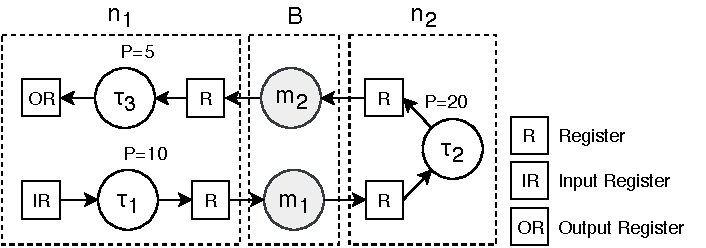
\includegraphics[width=0.7\linewidth]{img/cause_effect_chain_ntk}
	\caption{A Cause-effect Chain, mapped on nodes $n_1$ and $n_2$.}
	\label{fig_cause_effect_chain}
\end{figure}

The tasks $\tau_1$ and $\tau_2$ execute on node $n_1$, whereas task $\tau_3$ executes on node $n_2$. The execution time line of the chain over two hyper-periods are illustrated in Figure~\ref{fig_timedchainntk}. Note: $\tau_2$ communicates with $\tau_3$ via a CAN bus, which is not shown in the figure for simplicity. The red inverted arrows in the figure represent the reading of data from the input register, whereas the dashed-curve arrows represent the timed paths through which the data propagates from the input to the output of the chain. Thus, the age delay is the time elapsed between a stimulus arriving a the input register and its corresponding latest non-overwritten response at the output register, that is between the $3^{rd}$ instance of  $\tau_1$  and the $10^{th}$ instance of $\tau_3$. It is frequently used in the control systems applications where freshness of data is paramount, e.g., braking a car over a bounded time. And, the reaction delay is the earliest time the system takes to respond to a stimulus that ``just missed" the read access at the input of the chain. Assume that data arrives just after the start of the $1^{st}$ instance of $\tau_1$ execution. The data corresponding to this event is not read by the current instance of $\tau_1$. In fact, the data will be read by the $2^{nd}$ instance of $\tau_1$. The earliest effect of this data at the output of the chain will appear at the $7^{th}$ instance of $\tau_3$, which represents the reaction delay. This delay is useful in the body-electronics domain where first reaction to events is important, e.g., in the button-to-reaction applications. For detailed discussion of the different delay semantics, we direct the reader to check research work by Mubeen et al.~\cite{mubeen2013support}. 
\begin{figure}
	\centering
	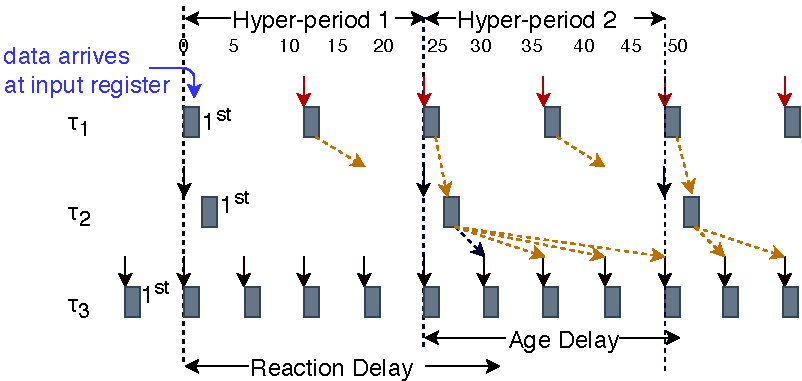
\includegraphics[width=0.9\linewidth]{img/timedchain_ntk}
	\caption{Reaction and Age Delays of the Cause-effect Chain, Shown in Figure {\ref{fig_causeeffectchainntk}}.}
	\label{fig_timedchainntk}
\end{figure}

The age delay is computed using Equation (\ref{eqn_agedelay_singlenode}) and Equation (\ref{eqn_agedelay_multinode}) for a single node and multiple nodes, respectively.

\begin{align}
	\label{eqn_agedelay_singlenode}
	\Delta^{sub}(\Gamma) &= \alpha(sink(\Gamma))-\alpha(source(\Gamma)) + \delta(sink(\Gamma)) & \text{single unit}\\
	\label{eqn_agedelay_multinode}
	\Delta(\Gamma)&=\sum_{i\in I_{\Gamma}}{\Delta^{sub}(i)} + \sum_{j\in  J_{\Gamma}}{\delta^{msg}(j)}, &\text{muliple units}
\end{align}
where $\alpha(\tau)$ computes the activation of the task $\tau$, based on the age-delay semanics.

Assume $\Gamma \in \ssp{\Gamma}$ is a chain, if the chain is mapped on a single computing unit, the age delay is a mere difference between the activation of the sink task $\ssb{\alpha}[\tau_j]$ and the activation of the source task $\ssb{\alpha}[\tau_i]$ plus the worst-case response time of the sink task $\ssb{\delta}[\tau_j]$ in the longest timed path according to the semantics of the age delay. On the other hand, if the chain is mapped to multiple nodes, the age delay $\Delta_{multi}$ can be compositionally computed~\cite{Feiertag2009ASemantics} as follows: the chain is partitioned  into a set of sub-chains per node, indicated by the predicate $subch(\Gamma)$, and for each sub-chain $a\in subch(\Gamma)$, the age delay is computed recursively using the same method to used to compute the age delay for a single node, and the result is added to the response-times of the messages involved in the chain, $msg(\Gamma)$.

\subsection{Reliability of Software Applications}\label{sub_reliability}
In this context, \textit{software application reliability} refers to the probability that a software application functions correctly by the time $t$, or within the time interval $[0, t]$ \cite{Goel1985SoftwareApplicability}. Redundancy is the most common way for implementing fault tolerance and increasing the reliability of a system. Redundancy can be implemented according to different schemes, such as hot stand-by, cold stand-by, etc.~\cite{Dubrova2013Fault-tolerantDesign}, which differ on the number of replicas that are active as well as the methods for detection and compensation of faulty replicas. In our system model, we consider the hot-standby scheme, where replicated components maintain the same state, but only one replica (the so-called \textit{primary}) effectively acts on the environment, for instance issuing an input. The primary software component will be denoted as \ttsss{q}[k][i,1], whereas the secondary software component, which is in the stand-by, by \ttsss{q}[k][i,2], etc., for a software application $A_k$.

%Note: the software components are replicated unless the reliability requirements of applications are satisfied.


In this work the details of the redundancy scheme are abstracted away under the following assumptions:
\begin{enumerate*}[label=(\roman*)]
    \item Software does not contain design errors. This has two implications: first, that hardware elements, i.e. computing nodes and communication buses, are the only causes of failure and, second, that introduction of N-version programming is not required. Different replicas of the same software component execute exactly the same program.
	\item Hot stand-by redundancy (also known as Primary/backup) is used for detection and replacement of failed components.
	\item Software components need to be replicated only if the application's reliability requirement is not met without replication, otherwise they are not replicated.
	\item The time needed to detect and replace a faulty component is considered negligible and will not be taken into account in the response time analysis of tasks and delay calculation of cause-effect chains;
	\item Because of its simplicity, the mechanism for detection and replacement of faulty components will be considered fault-free, and therefore will not be included in the reliability calculations
\end{enumerate*}

Note that under these assumptions, the reliability of a software application is equivalent to the reliability of the platform on which it is deployed. The reliability of a computing unit (and of the bus) can be easily calculated as $e^{\lambda t}$, where $\lambda$ is an exponentially distributed failure-rate. However, calculating the reliability of the whole execution platform is not trivial for the case with replication. In particular, the traditional series-parallel reliability approach cannot be applied because of the \textit{functional} interdependencies created between computing nodes as the result of replication and allocation. To illustrate the difficulty, let us assume a software application $A_k$, having  component configurations with and without replication as shown Table \ref{fig_depwr} and \ref{fig_depwor}, respectively, where $\sss{q}[k][i,j]$ is the $j^{th}$ software-component replica of software-component type $\sss{c}\in \sss{C}$. Note: for readability of the example, we remove the superscript $k$.
\begin{figure}
	\begin{subfigure}{.5\textwidth}
		\centering
		\begin{tabular}{ccc}
			$n_1$ & $n_2$ & $n_3$\\
			\hline
			\ttssb{q}[1,1]&\ttssb{q}[2,1]& \\
			\ttssb{q}[3,1]& & \\
			\hline
		\end{tabular}	
		\caption{Without Replication.}
		\label{fig_depwor}
	\end{subfigure}%
	\begin{subfigure}{.5\textwidth}
		\centering
		\begin{tabular}{ccc}
			$n_1$ & $n_2$ & $n_3$\\
			\hline
			\ttssb{q}[1,1]&\ttssb{q}[2,1]& \ttssb{q}[2,2]\\
			\ttssb{q}[3,1]& \ttssb{q}[1,2]& \ttssb{q}[3,2]\\
			\hline
		\end{tabular}
		\caption{With Replication.}
		\label{fig_depwr}
	\end{subfigure}%
	\caption{Partition of the Software Application $a_1$.}
	\label{fig_deployment}
\end{figure}

The reliability of the software application without replication forms a series path, indicated by the reliability block diagram (RBD) of Figure~\ref{fig_rbd}a, hence is computed as products of the reliability of $n_1,n_2$ and $B$. However, with replication, two computing nodes can form as series and parallel to service the software application,  e.g., due to \ttssb{q}[1,1] and \ttssb{q}[2,2] or \ttssb{q}[3,2], $n_1$ and $n_3$ make series, and due to \ttssb{q}[3,1] and \ttssb{q}[3,2], the nodes make parallel, to realize a partial functionality of the application. In this case, the series-parallel diagram depicted in Figure~\ref{fig_rbd}b does not accurately capture the reliability calculation of the application with replication. Note: the red-dashed line between $n_1$ and $n_3$ indicates the possibility of the computing nodes becoming series. To overcome this problem, we will use an exact technique for reliability calculation based on the enumeration of the different failure states of the computing nodes; that is, the different failure states of the execution platform are enumerated exhaustively, and subsequently, the total probability the software application functions is computed. This technique will be discussed in great length in Subsection~\ref{subsec_reliability_constraint}.
\begin{figure}
	\centering
	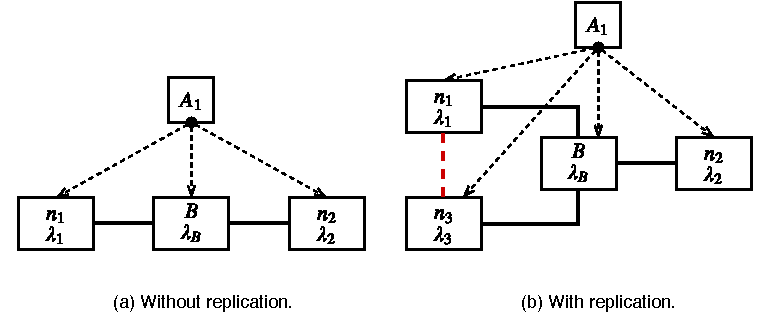
\includegraphics[width=0.8\linewidth]{img/rbd_replication}
	\caption{Reliability Block Diagrams of the Software Application.}
	\label{fig_rbd}
\end{figure}



